% Options for packages loaded elsewhere
\PassOptionsToPackage{unicode}{hyperref}
\PassOptionsToPackage{hyphens}{url}
\PassOptionsToPackage{dvipsnames,svgnames,x11names}{xcolor}
\documentclass[
  10pt,
  a4paper,
]{article}
\usepackage{xcolor}
\usepackage[margin=2.1cm]{geometry}
\usepackage{amsmath,amssymb}
\setcounter{secnumdepth}{-\maxdimen} % remove section numbering
\usepackage{iftex}
\ifPDFTeX
  \usepackage[T1]{fontenc}
  \usepackage[utf8]{inputenc}
  \usepackage{textcomp} % provide euro and other symbols
\else % if luatex or xetex
  \usepackage{unicode-math} % this also loads fontspec
  \defaultfontfeatures{Scale=MatchLowercase}
  \defaultfontfeatures[\rmfamily]{Ligatures=TeX,Scale=1}
\fi
\usepackage{lmodern}
\ifPDFTeX\else
  % xetex/luatex font selection
  \setmainfont[BoldFont=texgyreheros-bold.otf,ItalicFont=texgyreheros-italic.otf,BoldItalicFont=texgyreheros-bolditalic.otf]{texgyreheros-regular.otf}
  \setmonofont[BoldFont=texgyrecursor-bold.otf,Scale=0.9]{texgyrecursor-regular.otf}
\fi
% Use upquote if available, for straight quotes in verbatim environments
\IfFileExists{upquote.sty}{\usepackage{upquote}}{}
\IfFileExists{microtype.sty}{% use microtype if available
  \usepackage[]{microtype}
  \UseMicrotypeSet[protrusion]{basicmath} % disable protrusion for tt fonts
}{}
\makeatletter
\@ifundefined{KOMAClassName}{% if non-KOMA class
  \IfFileExists{parskip.sty}{%
    \usepackage{parskip}
  }{% else
    \setlength{\parindent}{0pt}
    \setlength{\parskip}{6pt plus 2pt minus 1pt}}
}{% if KOMA class
  \KOMAoptions{parskip=half}}
\makeatother
\usepackage{longtable,booktabs,array}
\usepackage{caption}
\captionsetup[table]{skip=6pt}
\newcounter{none} % for unnumbered tables
\usepackage{calc} % for calculating minipage widths
% Correct order of tables after \paragraph or \subparagraph
\usepackage{etoolbox}
\makeatletter
\patchcmd\longtable{\par}{\if@noskipsec\mbox{}\fi\par}{}{}
\makeatother
% Allow footnotes in longtable head/foot
\IfFileExists{footnotehyper.sty}{\usepackage{footnotehyper}}{\usepackage{footnote}}
\makesavenoteenv{longtable}
\usepackage{graphicx}
\makeatletter
\newsavebox\pandoc@box
\newcommand*\pandocbounded[1]{% scales image to fit in text height/width
  \sbox\pandoc@box{#1}%
  \Gscale@div\@tempa{\textheight}{\dimexpr\ht\pandoc@box+\dp\pandoc@box\relax}%
  \Gscale@div\@tempb{\linewidth}{\wd\pandoc@box}%
  \ifdim\@tempb\p@<\@tempa\p@\let\@tempa\@tempb\fi% select the smaller of both
  \ifdim\@tempa\p@<\p@\scalebox{\@tempa}{\usebox\pandoc@box}%
  \else\usebox{\pandoc@box}%
  \fi%
}
% Set default figure placement to htbp
\def\fps@figure{htbp}
\makeatother
\setlength{\emergencystretch}{3em} % prevent overfull lines
\providecommand{\tightlist}{%
  \setlength{\itemsep}{0pt}\setlength{\parskip}{0pt}}
\usepackage{etoolbox}\AtBeginEnvironment{longtable}{\footnotesize}
\usepackage{float}\floatplacement{figure}{H}
\setlength{\parskip}{5pt plus 1pt}\setlength{\parindent}{0pt}
\usepackage{caption}\captionsetup{font=small,skip=4pt,labelformat=empty}
\renewcommand{\arraystretch}{1.15}\usepackage{multicol}
\usepackage{bookmark}
\IfFileExists{xurl.sty}{\usepackage{xurl}}{} % add URL line breaks if available
\urlstyle{same}
% fallback for those not using the hyperref driver hyperxmp:
\makeatletter
\@ifundefined{xmpquote}{\newcommand{\xmpquote}[1]{#1}}{}
\makeatother
\hypersetup{
  pdftitle={Chinese ADR random-forest long-short},
  colorlinks=true,
  linkcolor={blue},
  filecolor={Maroon},
  citecolor={Blue},
  urlcolor={blue},
  pdfcreator={LaTeX via pandoc}}

\title{Chinese ADR random-forest long-short}
\author{}
\date{9 October 2026}

\begin{document}
\maketitle

Part I describes the model and the rule that turns its
forecasts into positions; Part II gives the backtest
statistics; the appendix lists the hyperparameters chosen
each year and the feature importances.

\section{Part I. Model
description}\label{part-i.-model-description}

\subsection{What it is}\label{what-it-is}

An application of a cross-sectional forecast of next-month
stock returns from ``Empirical Asset Pricing via Machine
Learning'' (Gu, Kelly, and Xiu, 2020), applied to the US
tradeable Chinese market. This strategy has exploitable
alpha primarily due to high borrow costs of rebalancing so
many short positions monthly forcing a capital constraint of
sub \$1M. Further evidence for this being the case is that
the same exact strategy run over US equities returns a
Sharpe of 0.13, demonstrating the decay of alpha within the
US domestic market, as this basic mechanism is undoubtedly
used to better effect domestically by various long-short
funds, which cannot enter our market due to the liquidity
constraint being too tight. The forecasts are turned into an
equal-weight long-short portfolio: long the top fifth of the
liquid universe, short the bottom fifth of the names that
trade at least \$10m a day. Nothing in the model uses
fundamentals, analysts, news or flows.

Headline result: on a \$500,000 account with a 10\%
volatility target, after commissions, borrow and cash
interest, the strategy grows to \$1.74m over January 2010 to
August 2026, a 7.7\% compound annual return at 10.8\%
volatility, Sharpe 0.75 on daily returns (0.86 monthly),
worst drawdown −19.3\%, with the money arriving in bursts
(2010--11, 2013, 2016--17, 2020--21, 2025--26) around flat
years. Before sizing, the dollar-neutral portfolio earns
36\% a year gross, Sharpe 1.02, of which the short leg
contributes −19\% a year and the long leg +17\%; it is close
to beta-neutral as well, with a beta of −0.15 and a
correlation of −0.13 to the PGJ China ETF (long leg beta
0.95, short leg 1.09).

\subsection{Universe}\label{universe}

US-listed Chinese companies (ADRs and direct listings)
assembled from the USCC lists of 2019, 2020 and 2025 and the
Nasdaq screener: 453 names over 2000--2026, 302 still
listed. Prices are dividend- and split-adjusted daily closes
with volume. Twelve SOEs that delisted in 2021--23 are
carried to their delisting dates through their Hong Kong
lines.

\subsection{Inputs}\label{inputs}

Daily prices are cleaned first: isolated prints that revert
the next day are dropped, both days of a crash-then-rebound
pair are removed, and any remaining single day above +300\%
(an unadjusted split) is removed. Then at each month-end t,
from that name's own history up to t:

{\def\LTcaptype{none} % do not increment counter
\begin{longtable}[]{@{}
  >{\raggedright\arraybackslash}p{(\linewidth - 2\tabcolsep) * \real{0.1575}}
  >{\raggedright\arraybackslash}p{(\linewidth - 2\tabcolsep) * \real{0.8425}}@{}}
\toprule\noalign{}
\begin{minipage}[b]{\linewidth}\raggedright
Characteristic
\end{minipage} & \begin{minipage}[b]{\linewidth}\raggedright
Definition
\end{minipage} \\
\midrule\noalign{}
\endhead
\bottomrule\noalign{}
\endlastfoot
ret\_1m & return over month t \\
mom\_6\_1, mom\_12\_1 & cumulative return over months
t−5..t−1 and t−11..t−1 \\
mom\_36\_13 & cumulative return over months t−35..t−12 \\
vol\_1m, vol\_3m & standard deviation of daily returns in
month t; average of the last three months' \\
ivol\_12m, beta\_12m & residual volatility and beta against
the equal-weight universe over the trailing 12 months of
daily returns \\
maxret\_1m, minret\_1m & largest and smallest daily return
in month t \\
dolvol\_1m & log of average daily dollar volume in month
t \\
dolvol\_trend & dolvol\_1m minus its trailing 12-month
mean \\
illiq\_1m & log Amihud ratio: mean of abs(return) / dollar
volume, \(\times\) 1e6 \\
zero\_1m & share of zero-return days in month t \\
high52 & month-end price divided by the 52-week high \\
age & log of months since first price \\
\end{longtable}
}

Each characteristic is converted to its percentile rank
within that month's tradeable cross-section (price \(\geq\)
\$1, \(\geq\) \$100k a day) and mapped to {[}−1, 1{]}; a
missing value becomes 0, the median. The model sees only
these sixteen ranks. Ranks must be computed over the same
kind of universe the model was fitted on: feeding it ranks
from a different universe (say, all US stocks) changes what
``+1 on dolvol\_1m'' means.

\subsection{Target}\label{target}

The next calendar month's return minus the 1-month T-bill.
For fitting only, the target is winsorised at the training
sample's 1st and 99th percentiles (about −0.45 and +0.71 for
the latest model).

\subsection{Estimator and refit
protocol}\label{estimator-and-refit-protocol}

A random forest of 300 trees, each split drawing on half of
the characteristics, with maximum tree depth in \{2, 4, 6\}
and minimum leaf size in \{20, 50\} chosen by validation
mean squared error. The protocol is an annual refit: in
December before test year Y, train on 2001..Y−3, validate on
Y−2..Y−1, pick the six-candidate winner, and use it
unchanged for the twelve months of Y. No test-year data
touches any fit. The hyperparameters chosen each year are
listed in Appendix A: shallow trees (depth 2) in most years
to 2019 and again for 2026, depth 4 to 6 in 2016--17 and
2020--25.

\subsection{What the forest has
learned}\label{what-the-forest-has-learned}

Impurity-based importance for the 2026 forest (Appendix B):
zero\_1m 0.33, high52 0.23, ivol\_12m 0.08, mom\_6\_1 0.05,
dolvol\_trend 0.05, minret\_1m 0.05, vol\_3m 0.05, ret\_1m
0.04, everything else below 0.04. The first thing the forest
does is separate names with many zero-return days (thin,
stale, often halted or about to be) from the rest, then it
reads price relative to the 52-week high, idiosyncratic
volatility and recent returns. The linear models fitted
alongside it in the research agree on the direction of the
stable terms: liquid, calm names near their highs score
high; thin, volatile, recently-collapsed names score low. In
the quintile sorts the short leg carries the result: the
bottom quintile of liquid names lost about 27\% a year over
2010--26, the top quintile earned about 14\% a year, roughly
what a volume-weighted index of the universe earned.

Forecast quality out of sample, 2010--26, all tradeable
names: R\(^2\) against a zero forecast 0.35\%, rank IC 0.080
(t 7.0), 0.081 on the liquid names (t 6.1).

\subsection{From forecasts to
positions}\label{from-forecasts-to-positions}

At each month-end, among tradeable names with \(\geq\) \$1m
a day (25 or more required, else flat): long the top
quintile by forecast, equal weight. Among those also trading
\(\geq\) \$10m a day (10 or more required, else flat): short
the bottom quintile, equal weight, at least five names. Hold
one calendar month, buy-and-hold inside it, re-form at the
next month-end. The \$10m floor is applied only here; the
model is fitted on the whole tradeable panel. Its purpose is
borrow: the thin third of the unrestricted short leg costs
more to borrow at retail than it earns, and removing it
leaves the spread intact.

Sizing in the \$500k backtest: dollars a side = min(80\%,
10\% \(\div\) \(\sigma\)) \(\times\) equity, resized
monthly, \(\sigma\) = 0.7 \(\times\) trailing 60-day
realised volatility of the one-dollar-a-side long-short +
0.3 \(\times\) its expanding mean. Fixed exposure (50\% a
side) earns about twice as much at one and a half times the
drawdown and the same Sharpe; the volatility target cut
exposure to 15--20\% a side in 2025--26 when the unit
volatility ran at 50--70\%.

\section{Part II. Backtest
statistics}\label{part-ii.-backtest-statistics}

All numbers are out of sample in the sense that no model saw
data from its test year; the design (features, universe,
model menu, the \$10m floor) was fixed with the research and
its literature in view. Window January 2010 to August 2026.

\subsection{1. Forecast quality}\label{forecast-quality}

All tradeable names, 2010--26.

{\def\LTcaptype{none} % do not increment counter
\begin{longtable}[]{@{}
  >{\raggedright\arraybackslash}p{(\linewidth - 6\tabcolsep) * \real{0.3878}}
  >{\raggedright\arraybackslash}p{(\linewidth - 6\tabcolsep) * \real{0.2449}}
  >{\raggedright\arraybackslash}p{(\linewidth - 6\tabcolsep) * \real{0.1122}}
  >{\raggedright\arraybackslash}p{(\linewidth - 6\tabcolsep) * \real{0.2551}}@{}}
\toprule\noalign{}
\begin{minipage}[b]{\linewidth}\raggedright
\end{minipage} & \begin{minipage}[b]{\linewidth}\raggedright
R\(^2\) vs zero forecast
\end{minipage} & \begin{minipage}[b]{\linewidth}\raggedright
Rank IC (t)
\end{minipage} & \begin{minipage}[b]{\linewidth}\raggedright
Rank IC, liquid names (t)
\end{minipage} \\
\midrule\noalign{}
\endhead
\bottomrule\noalign{}
\endlastfoot
Random forest & 0.35\% & 0.080 (7.0) & 0.081 (6.1) \\
Ensemble of five models, for reference & 0.31\% & 0.087
(8.2) & 0.089 (7.0) \\
Huber OLS, for reference & 0.44\% & 0.115 (9.7) & 0.107
(7.3) \\
\end{longtable}
}

\subsection{2. Quintile portfolios, unrestricted short
leg}\label{quintile-portfolios-unrestricted-short-leg}

Liquid universe (\(\geq\) \$1m a day), equal weight, 191
months, 62 names a month.

{\def\LTcaptype{none} % do not increment counter
\begin{longtable}[]{@{}
  >{\raggedright\arraybackslash}p{(\linewidth - 2\tabcolsep) * \real{0.3529}}
  >{\raggedright\arraybackslash}p{(\linewidth - 2\tabcolsep) * \real{0.6471}}@{}}
\toprule\noalign{}
\begin{minipage}[b]{\linewidth}\raggedright
\end{minipage} & \begin{minipage}[b]{\linewidth}\raggedright
Random forest
\end{minipage} \\
\midrule\noalign{}
\endhead
\bottomrule\noalign{}
\endlastfoot
Long-short return, annualised & +41.1\% \\
Long-short Sharpe, gross / net of 20 bp a side and 3\%
borrow & 1.16 / 0.93 (t 4.6) \\
Long-short worst drawdown & −37\% \\
Top quintile / bottom quintile excess return & +13.9\% /
−27.2\% a year \\
Equal-weight universe excess return & −1.5\% a year \\
Top quintile minus equal-weight universe, Sharpe & 0.89 \\
Turnover, long / short leg & 48\% / 58\% a month \\
Sub-period Sharpe 2010--15 / 2016--20 / 2021--26 & 1.31 /
0.99 / 1.19 \\
Calendar years, long-short gross (\%) & 2010 +33, 2011 +73,
2012 −4, 2013 +28, 2014 +36, 2015 +57, 2016 +53, 2017 +7,
2018 −17, 2019 −7, 2020 +226, 2021 +48, 2022 +23, 2023 +44,
2024 +54, 2025 +30, 2026 +82 (2026 to August) \\
\end{longtable}
}

\subsection{3. Borrow at retail scale and the \$10m
short-leg
rule}\label{borrow-at-retail-scale-and-the-10m-short-leg-rule}

Schedules by daily dollar volume, assumed not quoted: base
1\% above \$25m, 4\% at \$10--25m, 12\% at \$3--10m, 35\%
below \$3m; harsh 2 / 8 / 25 / 60\%.

{\def\LTcaptype{none} % do not increment counter
\begin{longtable}[]{@{}
  >{\raggedright\arraybackslash}p{(\linewidth - 10\tabcolsep) * \real{0.3443}}
  >{\raggedright\arraybackslash}p{(\linewidth - 10\tabcolsep) * \real{0.0984}}
  >{\raggedright\arraybackslash}p{(\linewidth - 10\tabcolsep) * \real{0.1148}}
  >{\raggedright\arraybackslash}p{(\linewidth - 10\tabcolsep) * \real{0.2049}}
  >{\raggedright\arraybackslash}p{(\linewidth - 10\tabcolsep) * \real{0.1230}}
  >{\raggedright\arraybackslash}p{(\linewidth - 10\tabcolsep) * \real{0.1148}}@{}}
\toprule\noalign{}
\begin{minipage}[b]{\linewidth}\raggedright
Short-leg rule
\end{minipage} & \begin{minipage}[b]{\linewidth}\raggedright
Gross Sharpe
\end{minipage} & \begin{minipage}[b]{\linewidth}\raggedright
Average borrow
\end{minipage} & \begin{minipage}[b]{\linewidth}\raggedright
Net Sharpe (base / harsh)
\end{minipage} & \begin{minipage}[b]{\linewidth}\raggedright
Net 2021--26
\end{minipage} & \begin{minipage}[b]{\linewidth}\raggedright
Shorts a month
\end{minipage} \\
\midrule\noalign{}
\endhead
\bottomrule\noalign{}
\endlastfoot
All liquid names, flat 3\% borrow & 1.19 & 3\% & 0.96 & 1.00
& 12 \\
All liquid names, tiered & 1.19 & 16 / 29\% & 0.60 / 0.24 &
0.68 / 0.36 & 12 \\
Names above \$3m a day & 1.37 & 7 / 14\% & 1.02 / 0.81 &
1.18 / 1.00 & 9 \\
\textbf{Names above \$10m a day (exported rule)} &
\textbf{1.04} & \textbf{2 / 5\%} & \textbf{0.84 / 0.77} &
\textbf{0.91 / 0.84} & \textbf{7} \\
Names above \$25m a day & 0.50 & 1 / 2\% & 0.35 / 0.33 &
0.39 / 0.36 & 6 \\
Long leg, short PGJ at 1\% & 0.53 & 1\% & 0.36 & −0.07 & \\
\end{longtable}
}

\subsection{4. The \$500,000 account,
2010--26}\label{the-500000-account-201026}

Daily P\&L on the monthly holdings; dollars a side =
min(80\%, 10\% \(\div\) \(\sigma\)) \(\times\) equity with
\(\sigma\) from the unit long-short's 60-day volatility
blended with its long-run mean; 20 bp a side; borrow per
name by volume; free cash at the bill less 0.5\%, short
proceeds above \$100k at the bill less 1.25\%; Reg T margin.

{\def\LTcaptype{none} % do not increment counter
\begin{longtable}[]{@{}
  >{\raggedright\arraybackslash}p{(\linewidth - 4\tabcolsep) * \real{0.3363}}
  >{\raggedright\arraybackslash}p{(\linewidth - 4\tabcolsep) * \real{0.4933}}
  >{\raggedright\arraybackslash}p{(\linewidth - 4\tabcolsep) * \real{0.1704}}@{}}
\toprule\noalign{}
\begin{minipage}[b]{\linewidth}\raggedright
\end{minipage} & \begin{minipage}[b]{\linewidth}\raggedright
Random forest (headline)
\end{minipage} & \begin{minipage}[b]{\linewidth}\raggedright
Same account on the ensemble forecasts
\end{minipage} \\
\midrule\noalign{}
\endhead
\bottomrule\noalign{}
\endlastfoot
Final equity from \$500,000 & \textbf{\$1.74m} & \$1.56m \\
CAGR / volatility & \textbf{7.7\% / 10.8\%} & 7.1\% /
10.7\% \\
Sharpe, daily / monthly & \textbf{0.75 / 0.86} & 0.70 /
0.76 \\
Worst drawdown & −19.3\% (Nov 2017 to Mar 2019, recovered
Jun 2020) & −16.6\% \\
Worst month / hit rate & −8.4\% / 57\% & −8.3\% / 55\% \\
Sub-period Sharpe 2010--15 / 2016--20 / 2021--26 & 0.78 /
0.61 / 0.86 & 0.57 / 0.63 / 0.87 \\
Exposure a side, average (range) & 28\% (12 to 44\%) &
28\% \\
Margin pledged, average / peak (Reg T initial); maintenance
peak; call days & 28\% / 49\%; 27\%; 0 & \\
Commissions and spread / borrow (2.3\% a year) / cash
interest earned & \$224k / \$95k / +\$211k & \\
Flat months (too few names) & 11 (Dec 2009, Jul 2010, Dec
2011, May 2012, Jun 2012, Jul 2012, Aug 2012, Sep 2012, Oct
2012, Nov 2012, Feb 2013) & \\
\end{longtable}
}

\begin{figure}
\centering
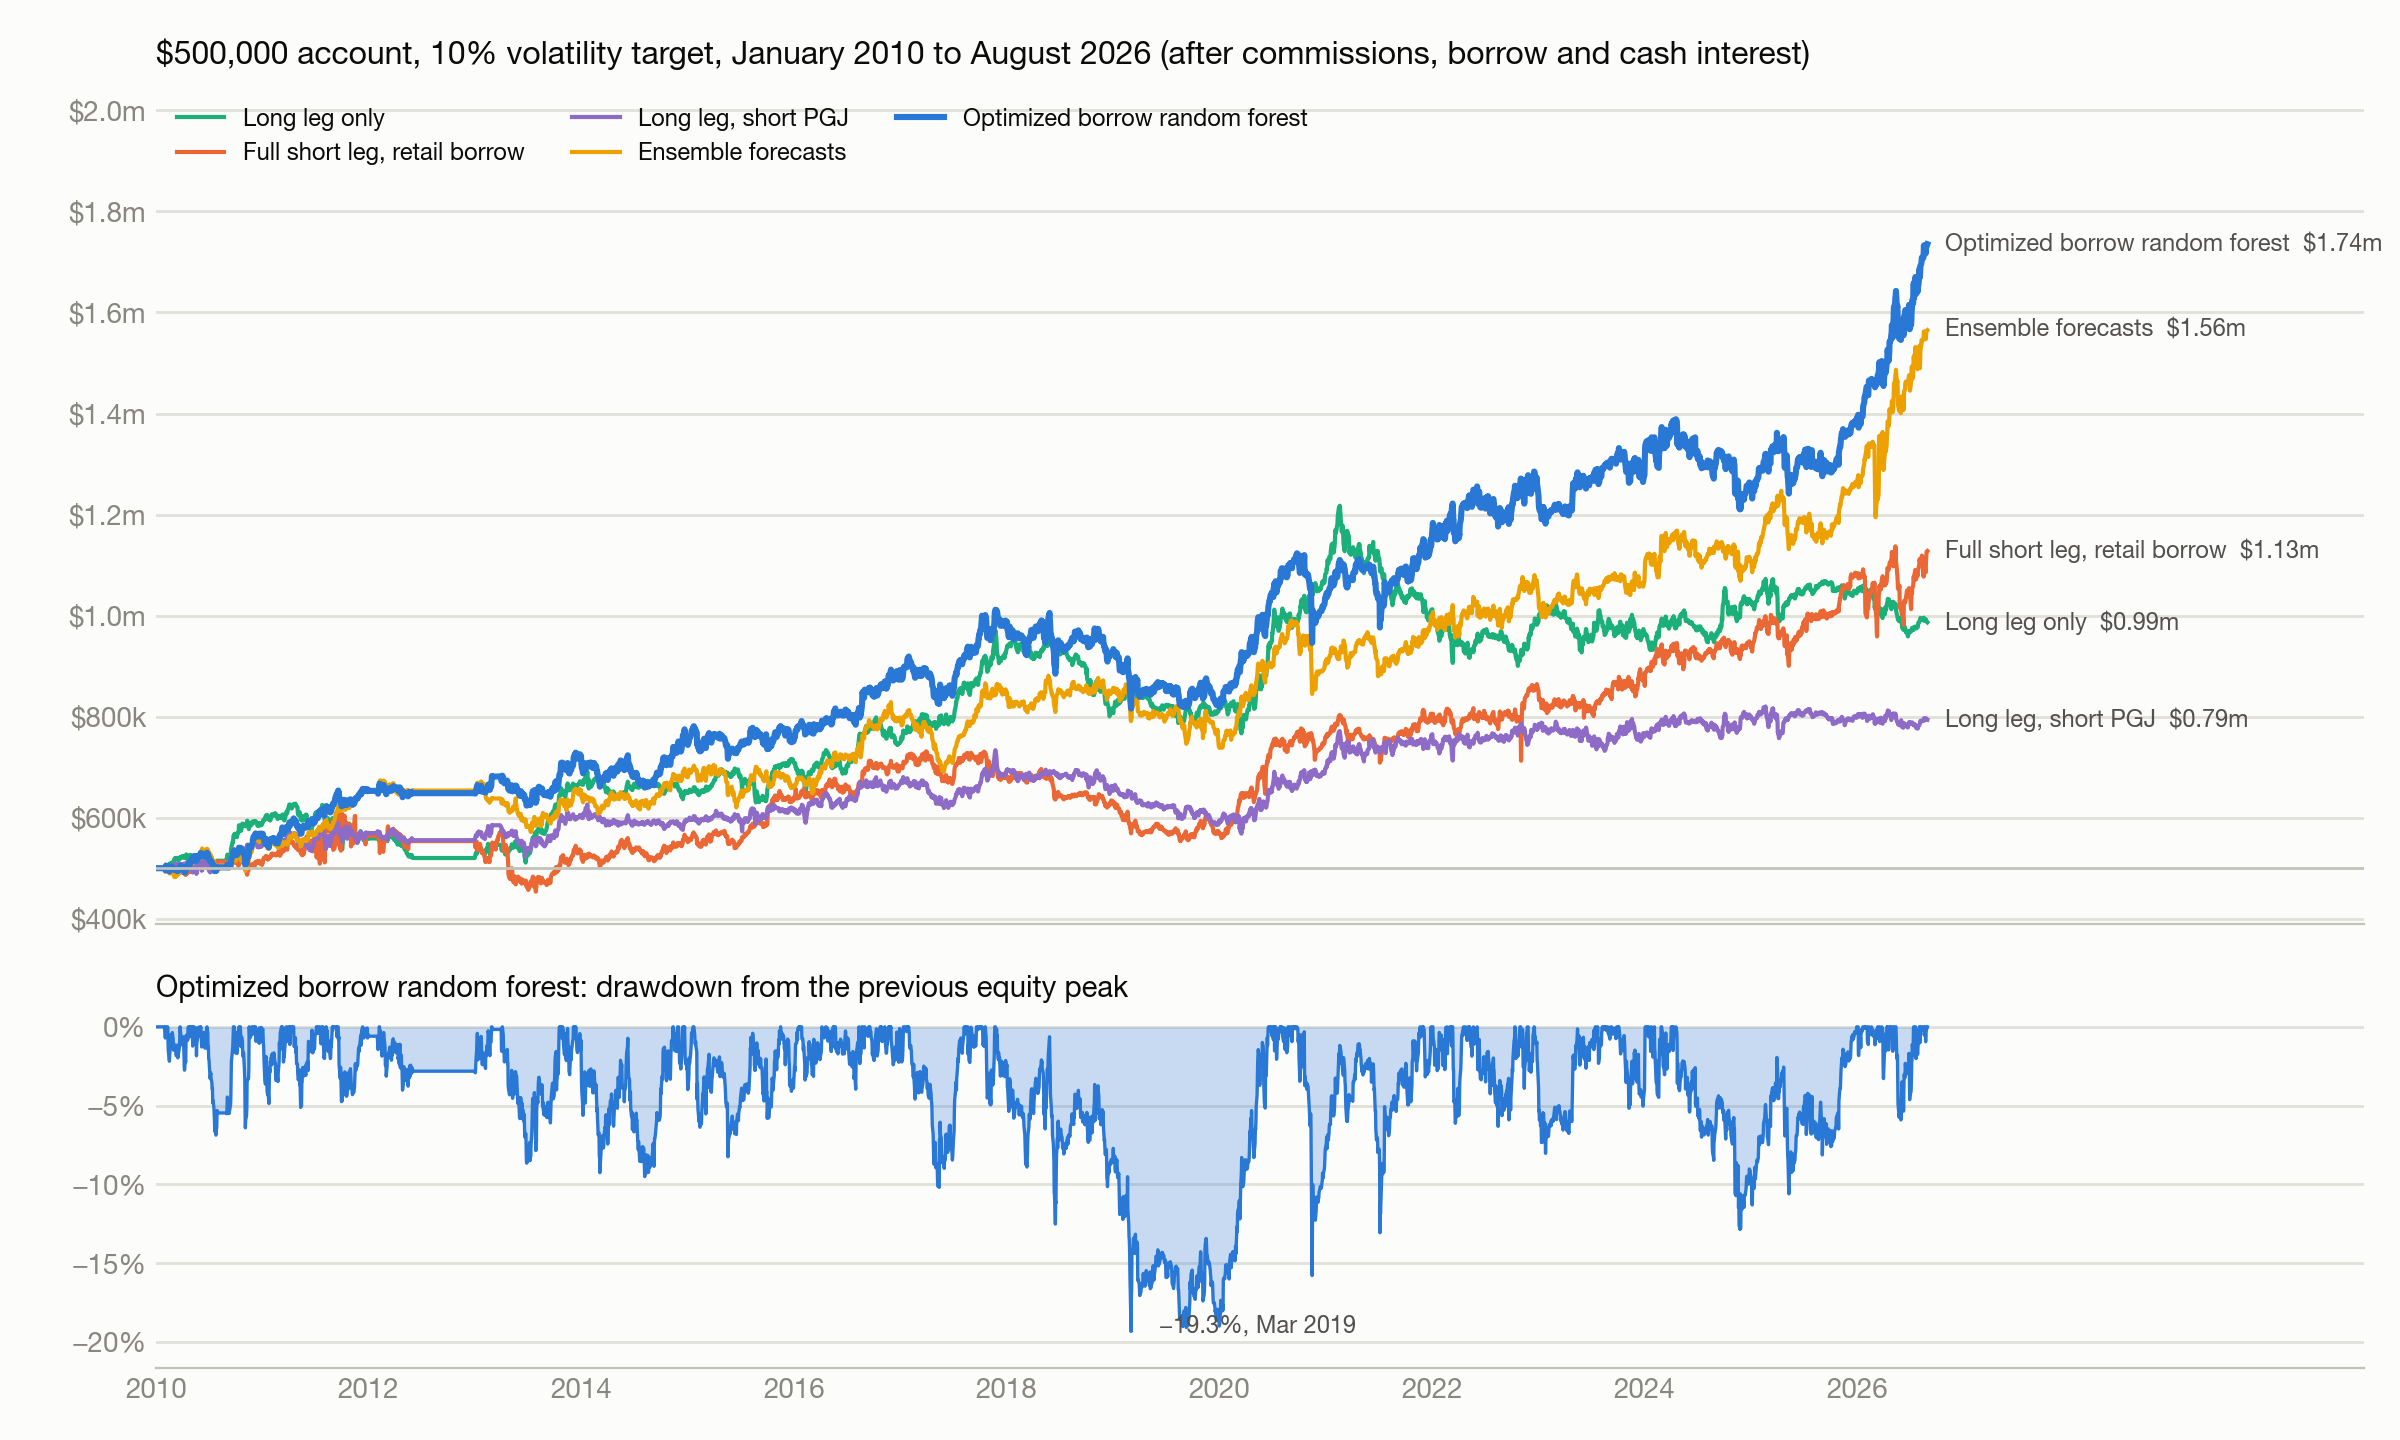
\includegraphics[width=1\linewidth,height=\textheight,keepaspectratio,alt={Figure 2. Account equity and drawdown, January 2010 to August 2026: the optimized-borrow random forest against the same account on the ensemble forecasts, the full short leg at retail borrow, the long leg alone and the long leg hedged with PGJ.}]{results/fig2_bt500k_rf_equity.png}
\caption{Figure 2. Account equity and drawdown, January 2010
to August 2026: the optimized-borrow random forest against
the same account on the ensemble forecasts, the full short
leg at retail borrow, the long leg alone and the long leg
hedged with PGJ.}
\end{figure}

Calendar years, return on the account (\%): 2010 +13.6, 2011
+15.4, 2012 −0.6, 2013 +11.6, 2014 +4.6, 2015 −0.7, 2016
+18.8, 2017 +11.0, 2018 −6.4, 2019 −10.6, 2020 +25.1, 2021
+10.7, 2022 +9.6, 2023 +1.1, 2024 −0.8, 2025 +10.4, 2026
+24.8 (2026 to August). The best five months are 28\% of the
P\&L, the best ten 50\%.

Sizing and cost variants (final equity, CAGR, Sharpe daily,
worst drawdown): 15\% vol target \$2.80m, 10.9\%, 0.72,
−28\%; 20\% target \$4.38m, 13.9\%, 0.71, −37\%; fixed 50\%
a side \$4.18m, 13.5\%, 0.74, −31\%; fixed 80\% a side
\$10.61m, 20.1\%, 0.73, −46\% with 0 margin-call days; harsh
borrow 0.69; flat 8\% borrow 0.60; no borrow 0.81; 10 bp
costs 0.82; 40 bp costs 0.62.

Other legs on the same account: full short leg at retail
borrow (16\% a year) \$1.13m, Sharpe 0.38; short leg above
\$25m \$815k, 0.34; long leg alone \$987k, 0.48; long leg
hedged with PGJ \$794k, 0.34.

\subsection{5. Monte Carlo and
nulls}\label{monte-carlo-and-nulls}

\begin{figure}
\centering
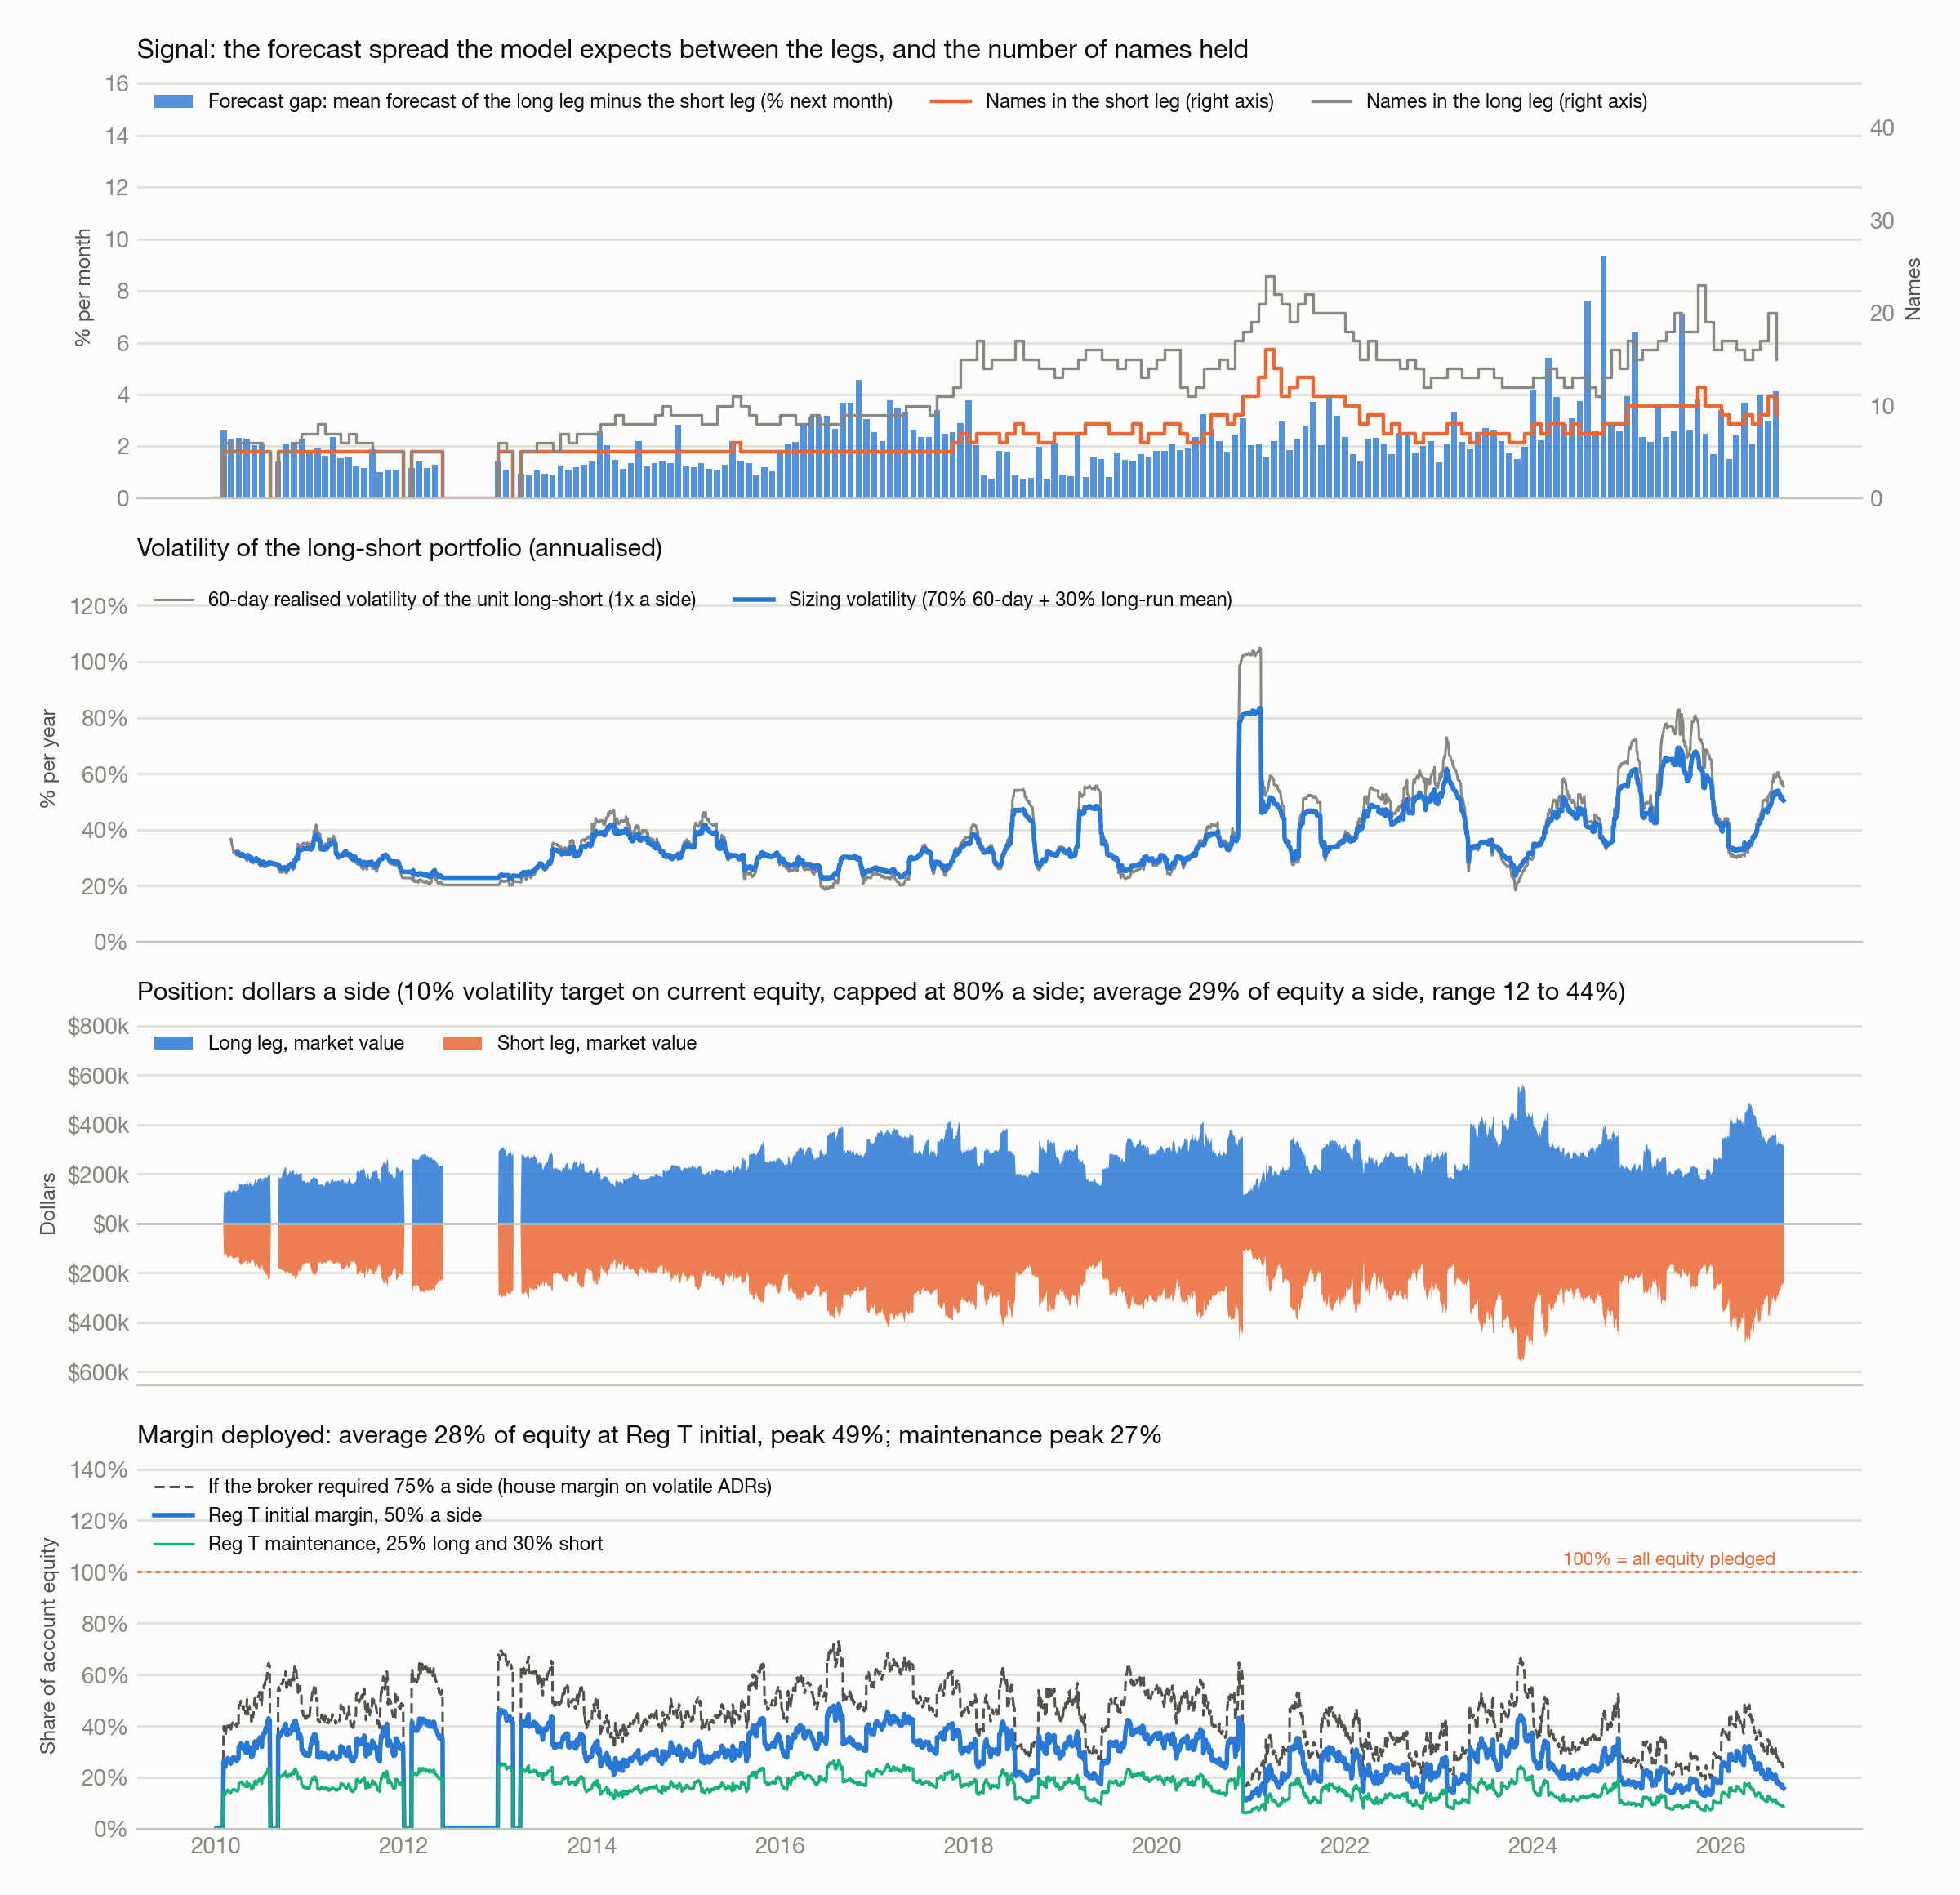
\includegraphics[width=\linewidth,height=0.88\textheight,keepaspectratio,alt={Figure 3. Signal (forecast gap and names held), volatility of the long-short, dollars a side, and margin deployed, 2010 to 2026.}]{results/fig3_bt500k_rf_signal_vol_margin.png}
\caption{Figure 3. Signal (forecast gap and names held),
volatility of the long-short, dollars a side, and margin
deployed, 2010 to 2026.}
\end{figure}

\begin{figure}
\centering
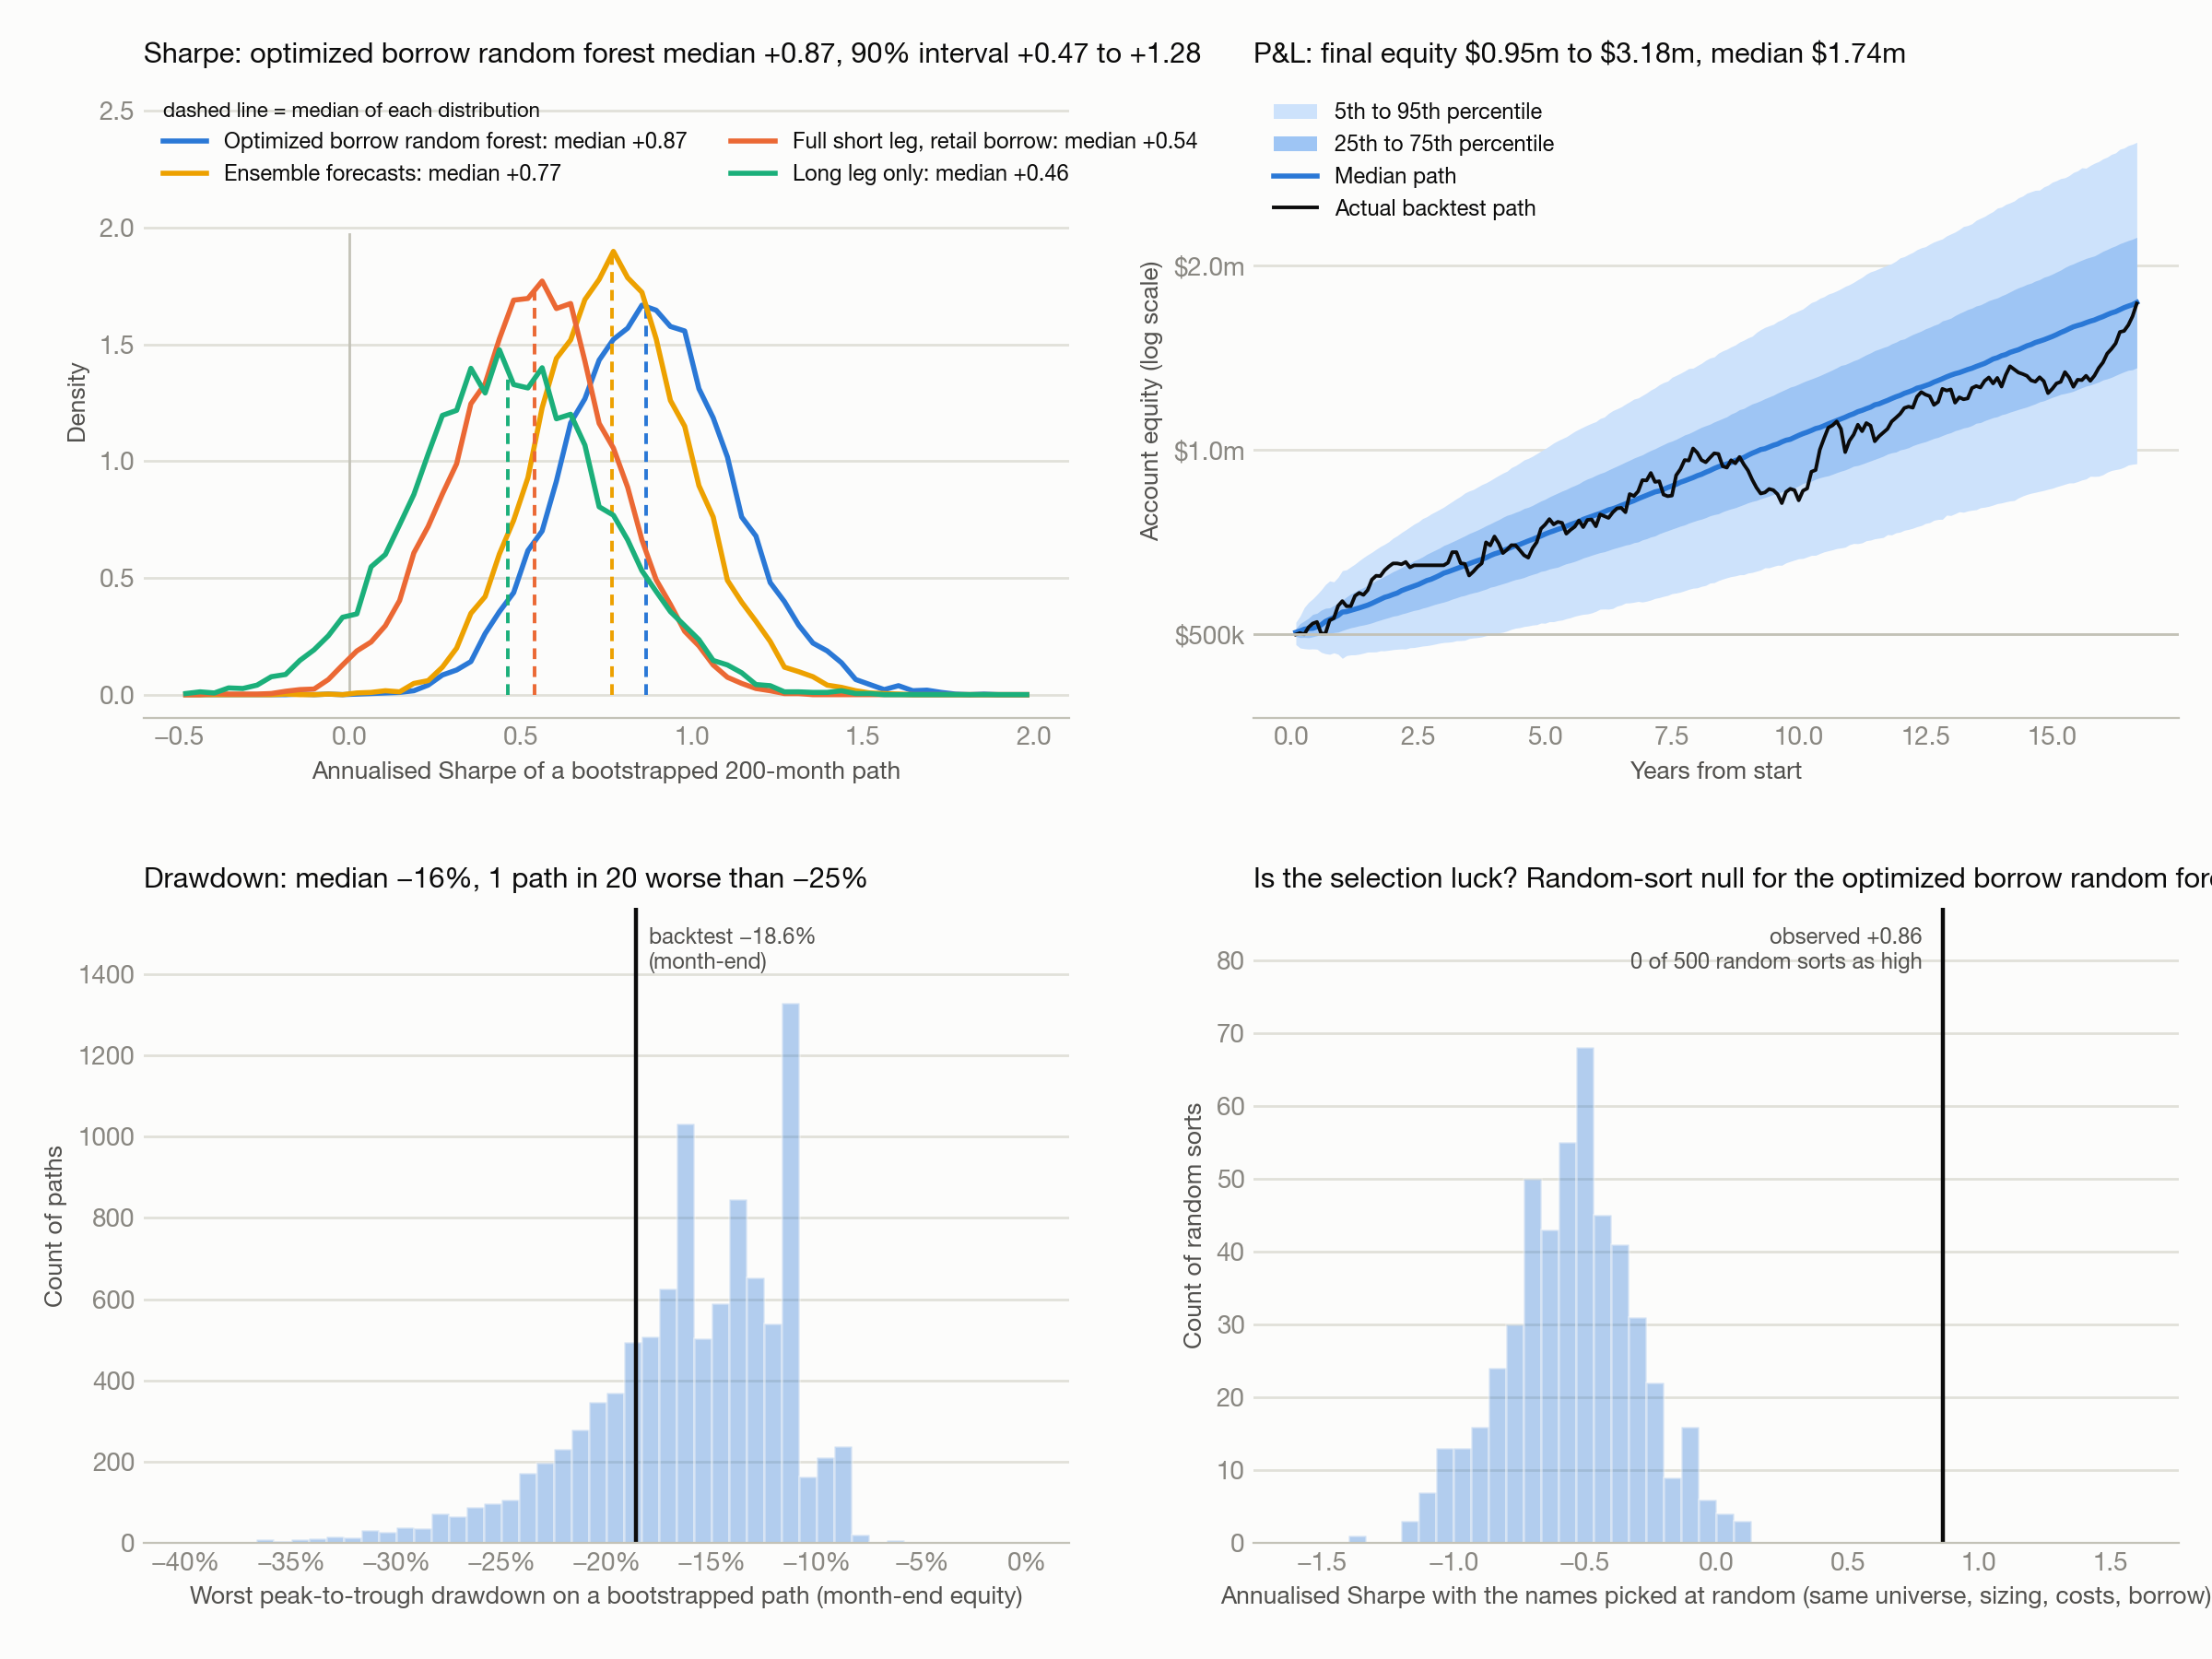
\includegraphics[width=1\linewidth,height=\textheight,keepaspectratio,alt={Figure 4. Bootstrap Sharpe densities, equity fan against the actual path, drawdown distribution, and the random-sort null.}]{results/fig4_bt500k_rf_montecarlo.png}
\caption{Figure 4. Bootstrap Sharpe densities, equity fan
against the actual path, drawdown distribution, and the
random-sort null.}
\end{figure}

\subsection{6. The last five years as a fresh
account}\label{the-last-five-years-as-a-fresh-account}

\begin{figure}
\centering
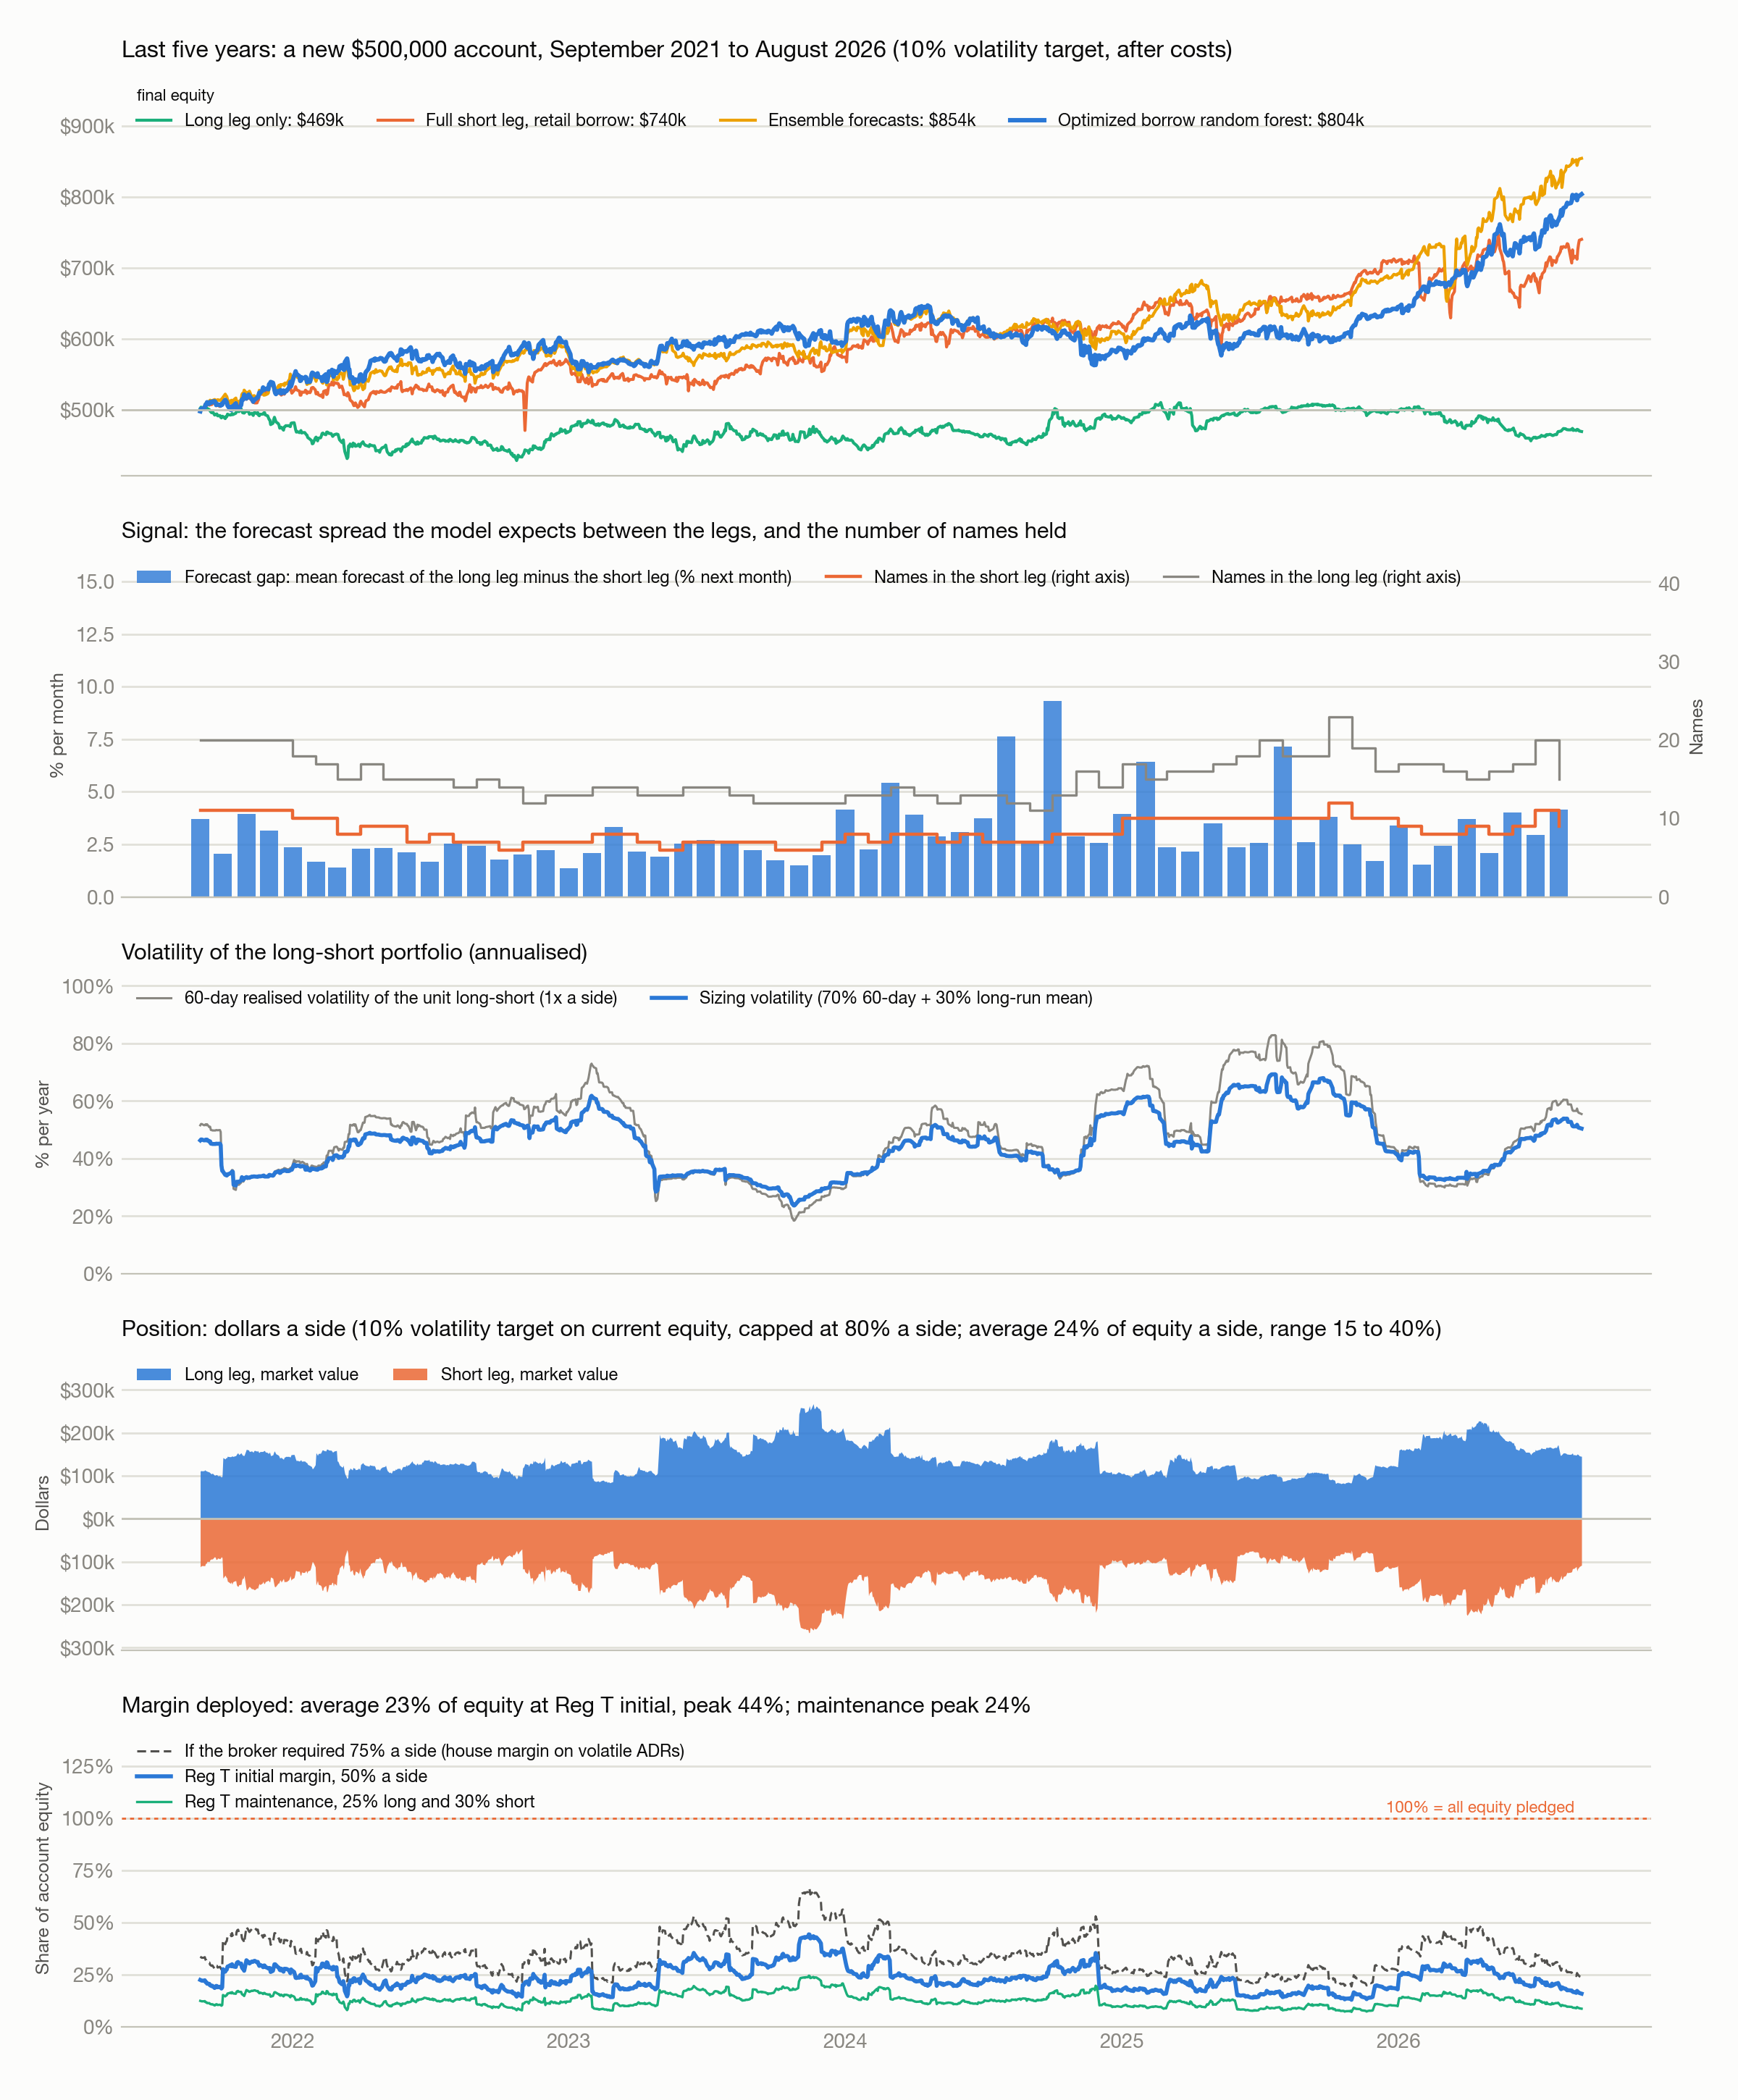
\includegraphics[width=\linewidth,height=0.88\textheight,keepaspectratio,alt={Figure 5. A fresh account from September 2021: equity, signal, volatility, dollars a side, margin.}]{results/fig5_bt500k_rf_5y_account.png}
\caption{Figure 5. A fresh account from September 2021:
equity, signal, volatility, dollars a side, margin.}
\end{figure}

\begin{figure}
\centering
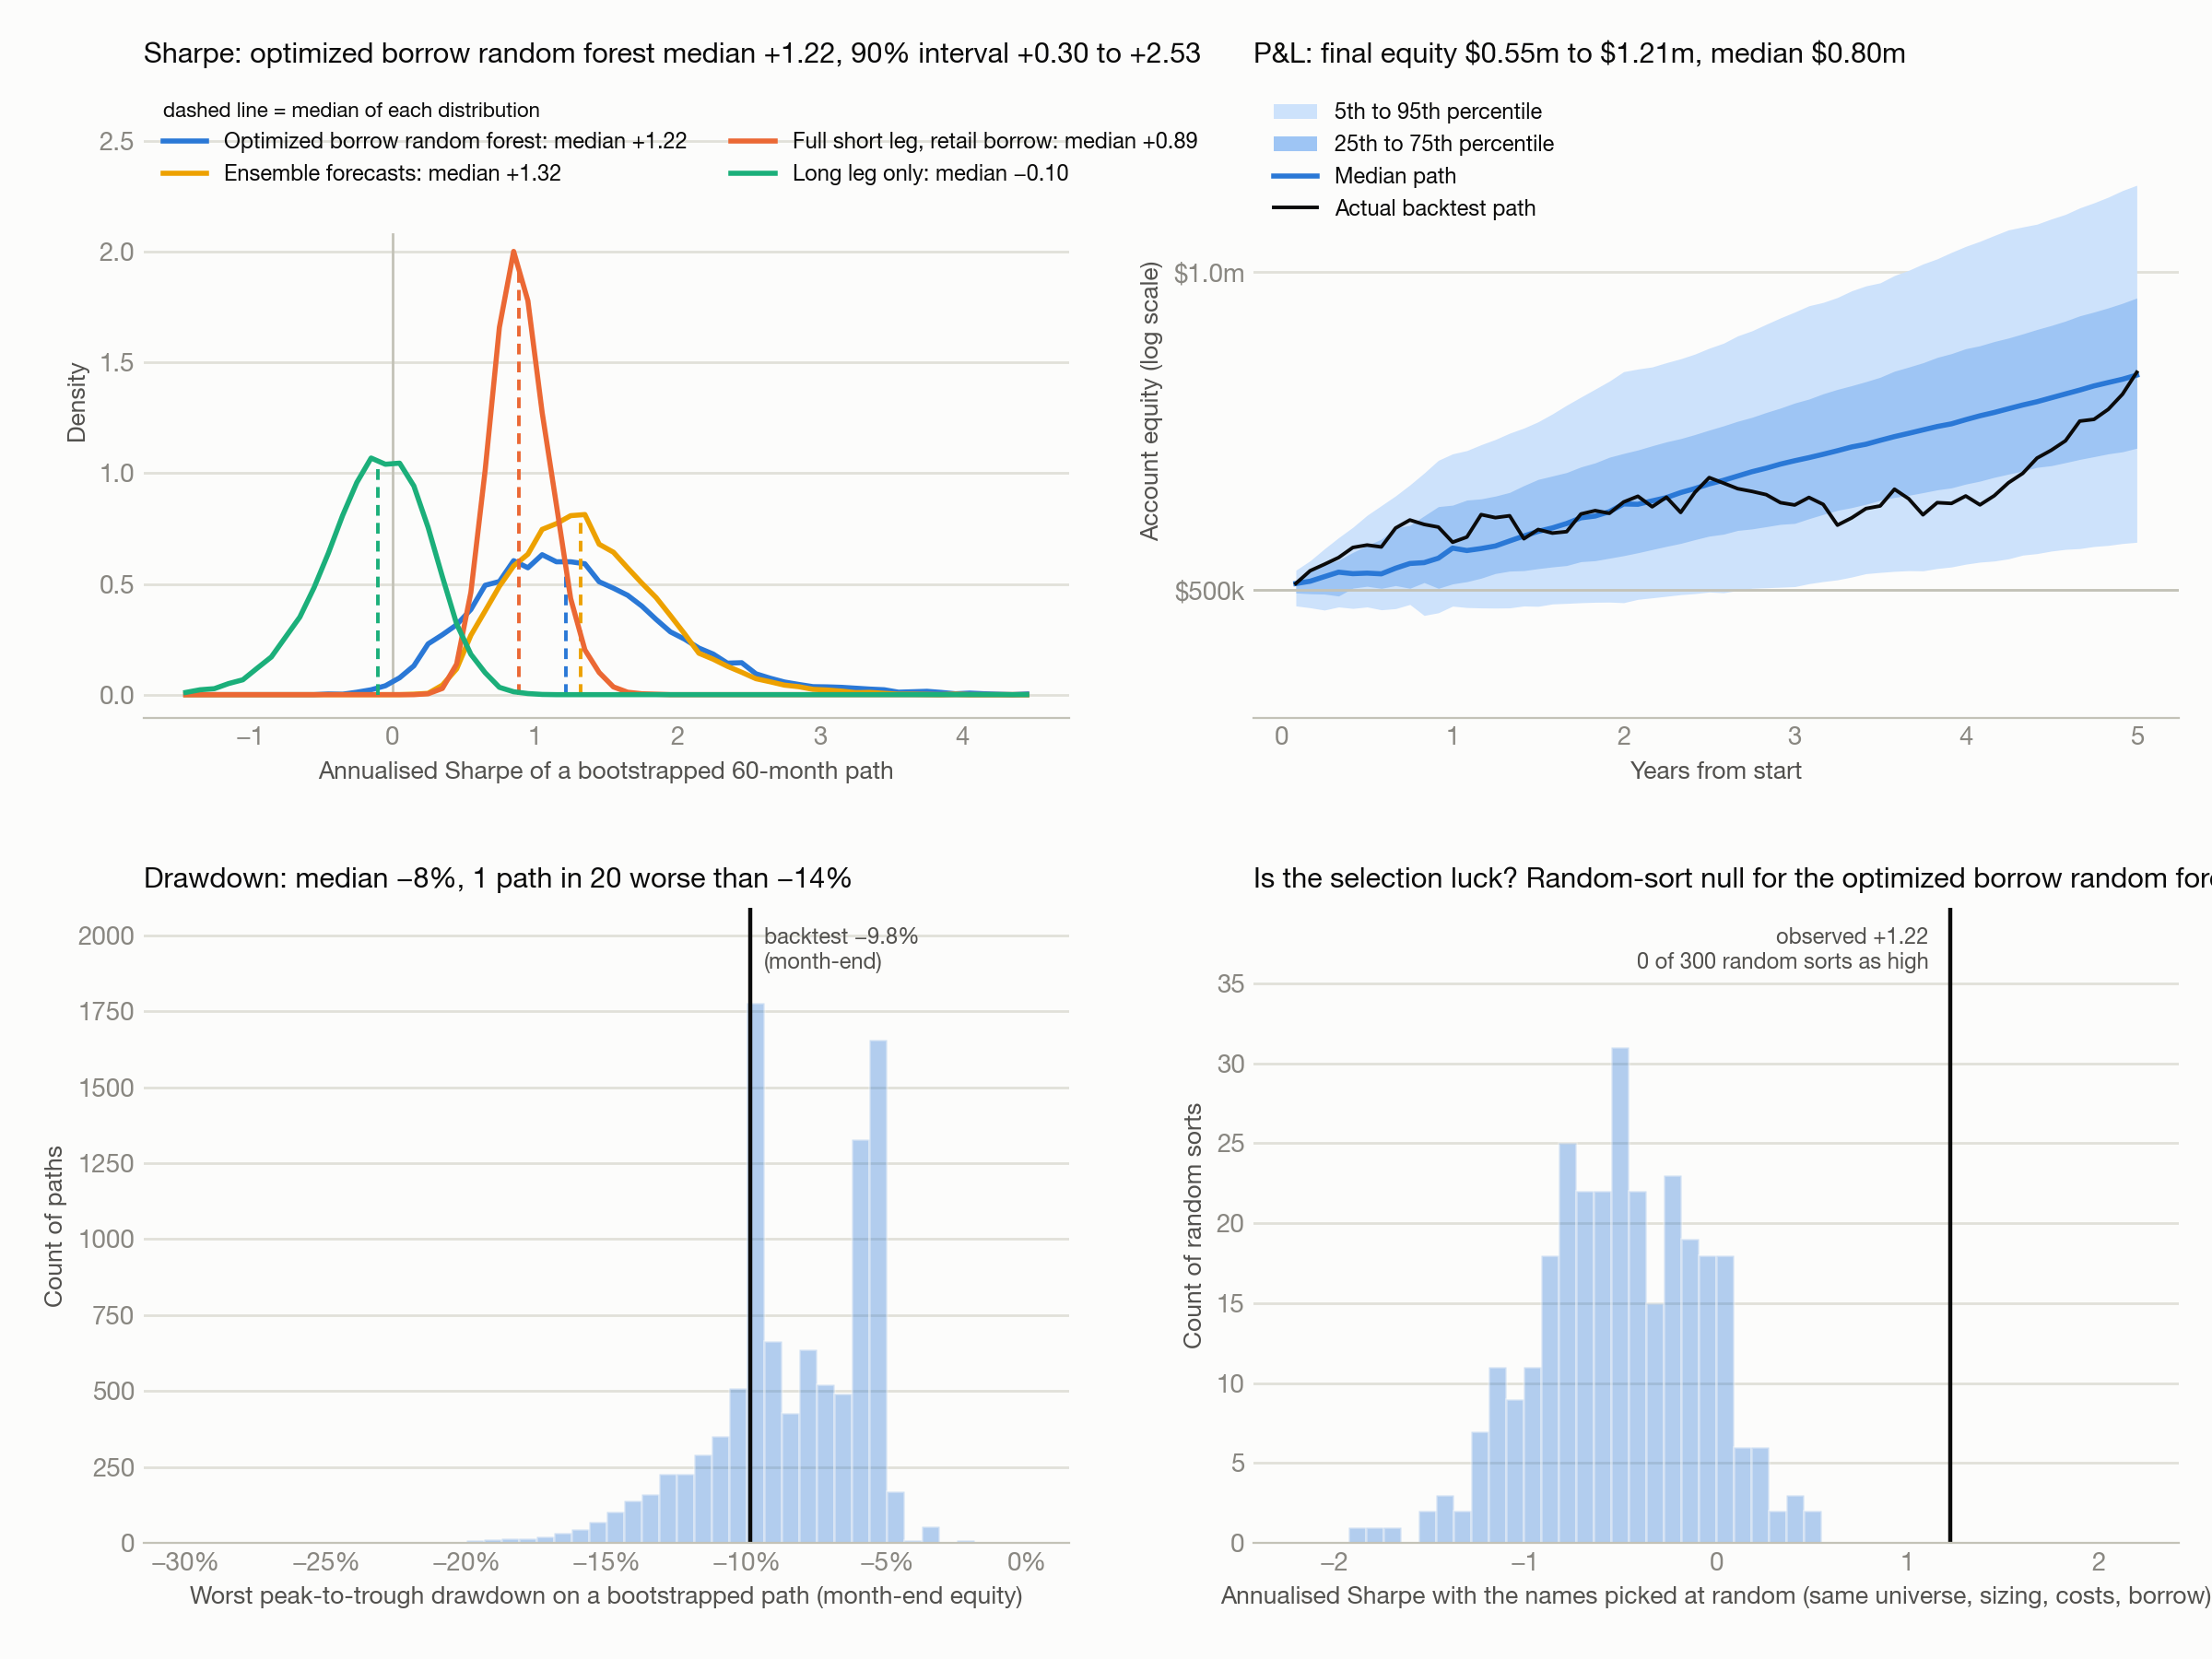
\includegraphics[width=1\linewidth,height=\textheight,keepaspectratio,alt={Figure 6. Monte Carlo on the 60 months.}]{results/fig6_bt500k_rf_5y_montecarlo.png}
\caption{Figure 6. Monte Carlo on the 60 months.}
\end{figure}

\subsection{7. Cross-checks and
limits}\label{cross-checks-and-limits}

\begin{itemize}
\tightlist
\item
  Price data: Yahoo and an independent archive agree on
  99.95\% of overlapping stock-months. Two data bugs were
  found and fixed in review (an asymmetric return filter
  that turned bad prints into −100\% months, and a
  label-indexing error in the cleaning step that nulled
  unrelated days when sources were concatenated); the
  numbers here are from the corrected pipeline.
\item
  Survivorship: names that delisted after April 2020, other
  than twelve SOEs carried through Hong Kong, are missing
  for their final months. The volume-weighted universe
  correlates 0.92 with PGJ and trails it by 4\% a year in
  2021--26, so the survivor premium is not driving the
  recent numbers; the small-cap delistings sit in the short
  leg and remain unmeasured.
\item
  Concentration: the pool above \$10m a day was 10 to 25
  names until 2017, so the short leg was its minimum of five
  names; it has been 7 to 12 since 2018.
\end{itemize}

\section{Appendix}\label{appendix}

\subsection{A. Hyperparameters chosen by validation, by test
year}\label{a.-hyperparameters-chosen-by-validation-by-test-year}

Each December before test year Y the forest is trained on
2001..Y−3 and the six candidates (max\_depth 2, 4, 6
\(\times\) min\_samples\_leaf 20, 50) are scored on
Y−2..Y−1. Refitting with these settings reproduces the saved
forecasts to machine precision.

{\def\LTcaptype{none} % do not increment counter
\begin{longtable}[]{@{}
  >{\raggedright\arraybackslash}p{(\linewidth - 10\tabcolsep) * \real{0.1071}}
  >{\raggedright\arraybackslash}p{(\linewidth - 10\tabcolsep) * \real{0.2500}}
  >{\raggedright\arraybackslash}p{(\linewidth - 10\tabcolsep) * \real{0.1786}}
  >{\raggedright\arraybackslash}p{(\linewidth - 10\tabcolsep) * \real{0.1071}}
  >{\raggedright\arraybackslash}p{(\linewidth - 10\tabcolsep) * \real{0.1905}}
  >{\raggedright\arraybackslash}p{(\linewidth - 10\tabcolsep) * \real{0.1667}}@{}}
\toprule\noalign{}
\begin{minipage}[b]{\linewidth}\raggedright
Test year
\end{minipage} & \begin{minipage}[b]{\linewidth}\raggedright
Training rows (names)
\end{minipage} & \begin{minipage}[b]{\linewidth}\raggedright
Validation rows
\end{minipage} & \begin{minipage}[b]{\linewidth}\raggedright
max\_depth
\end{minipage} & \begin{minipage}[b]{\linewidth}\raggedright
min\_samples\_leaf
\end{minipage} & \begin{minipage}[b]{\linewidth}\raggedright
Validation MSE
\end{minipage} \\
\midrule\noalign{}
\endhead
\bottomrule\noalign{}
\endlastfoot
2010 & 1,657 (41) & 907 & 2 & 20 & 0.0333 \\
2011 & 2,097 (47) & 1,065 & 2 & 50 & 0.0252 \\
2012 & 2,564 (54) & 1,270 & 2 & 50 & 0.0254 \\
2013 & 3,162 (68) & 1,271 & 2 & 20 & 0.0250 \\
2014 & 3,834 (73) & 1,300 & 2 & 50 & 0.0235 \\
2015 & 4,433 (77) & 1,563 & 2 & 20 & 0.0237 \\
2016 & 5,134 (80) & 1,711 & 6 & 50 & 0.0236 \\
2017 & 5,996 (90) & 1,757 & 6 & 50 & 0.0209 \\
2018 & 6,845 (100) & 1,971 & 2 & 20 & 0.0216 \\
2019 & 7,753 (115) & 2,468 & 2 & 50 & 0.0283 \\
2020 & 8,816 (138) & 2,964 & 4 & 50 & 0.0300 \\
2021 & 10,221 (173) & 2,918 & 4 & 50 & 0.0374 \\
2022 & 11,780 (201) & 3,105 & 4 & 50 & 0.0427 \\
2023 & 13,139 (226) & 3,166 & 6 & 50 & 0.0457 \\
2024 & 14,885 (248) & 2,722 & 6 & 20 & 0.0461 \\
2025 & 16,305 (256) & 2,754 & 4 & 20 & 0.0441 \\
2026 & 17,607 (276) & 3,315 & 2 & 20 & 0.0488 \\
\end{longtable}
}

\subsection{B. Impurity-based feature
importance}\label{b.-impurity-based-feature-importance}

{\def\LTcaptype{none} % do not increment counter
\begin{longtable}[]{@{}lll@{}}
\toprule\noalign{}
Characteristic & rf\_2026 & rf\_next \\
\midrule\noalign{}
\endhead
\bottomrule\noalign{}
\endlastfoot
zero\_1m & 0.326 & 0.291 \\
high52 & 0.231 & 0.076 \\
ivol\_12m & 0.082 & 0.072 \\
mom\_6\_1 & 0.051 & 0.044 \\
dolvol\_trend & 0.051 & 0.037 \\
minret\_1m & 0.050 & 0.057 \\
vol\_3m & 0.046 & 0.061 \\
ret\_1m & 0.043 & 0.063 \\
beta\_12m & 0.027 & 0.050 \\
maxret\_1m & 0.024 & 0.041 \\
mom\_12\_1 & 0.022 & 0.033 \\
dolvol\_1m & 0.015 & 0.042 \\
age & 0.011 & 0.040 \\
illiq\_1m & 0.010 & 0.034 \\
vol\_1m & 0.008 & 0.038 \\
mom\_36\_13 & 0.003 & 0.021 \\
\end{longtable}
}

\end{document}
